\documentclass[tikz,border=3pt]{standalone}
\usepackage[utf8]{inputenc}
\usepackage[T1]{fontenc}
\usepackage{lmodern}
\renewcommand{\familydefault}{\sfdefault}
\usepackage{amsmath}
\usepackage{sansmath}\sansmath
\usepackage{pgfplots}\pgfplotsset{compat=1.18,/pgf/number format/use comma,/pgf/number format/1000 sep={.}}
\usetikzlibrary{arrows.meta,calc,positioning,decorations.pathmorphing,patterns}
% paleta del sitio
\definecolor{nar}{HTML}{E8680C}\definecolor{narc}{HTML}{FFB35C}\definecolor{hielo}{HTML}{FFF3E8}
\definecolor{tinta}{HTML}{1D1D1F}\definecolor{gris}{HTML}{6E6E73}\definecolor{lila}{HTML}{7C5CF0}
\definecolor{azul}{HTML}{2F6FD6}\definecolor{menta}{HTML}{17A673}\definecolor{coral}{HTML}{E8342A}
\pgfplotsset{base/.style={axis lines=left,grid=major,grid style={gris!20},tick label style={font=\small},label style={font=\small},axis line style={tinta!80}}}
\begin{document}
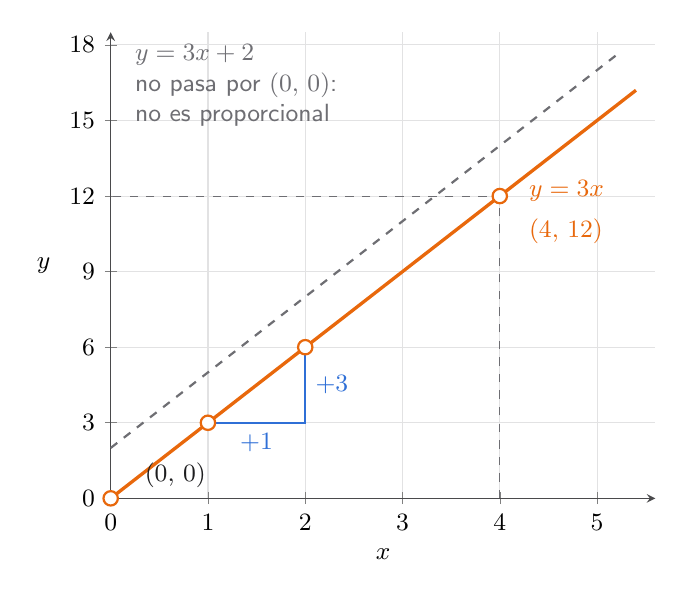
\begin{tikzpicture}
\begin{axis}[base,width=8.5cm,height=7.5cm,xmin=0,xmax=5.6,ymin=0,ymax=18.5,xtick={0,...,5},ytick={0,3,...,18},xlabel={$x$},ylabel={$y$},ylabel style={rotate=-90},clip=false]
\addplot[gris,thick,dashed,domain=0:5.2] {3*x+2};
\addplot[nar,very thick,domain=0:5.4] {3*x};
\draw[gris,dashed] (axis cs:4,0) -- (axis cs:4,12) -- (axis cs:0,12);
\draw[azul,thick] (axis cs:1,3) -- (axis cs:2,3) node[midway,below,font=\small]{$+1$} -- (axis cs:2,6) node[midway,right,font=\small]{$+3$};
\addplot[only marks,mark=*,mark options={fill=white,draw=nar,thick},mark size=2.6pt] coordinates {(0,0)(1,3)(2,6)(4,12)};
\node[nar,font=\small\bfseries,anchor=west] at (axis cs:4.2,12.2) {$y = 3x$};
\node[nar,font=\small,anchor=west] at (axis cs:4.2,10.6) {$(4,\,12)$};
\node[gris,font=\small,anchor=north west,align=left] at (axis cs:0.15,18.4) {$y = 3x + 2$\\no pasa por $(0,\,0)$:\\no es proporcional};
\node[tinta,font=\small,anchor=west] at (axis cs:0.25,0.9) {$(0,\,0)$};
\end{axis}
\end{tikzpicture}
\end{document}
